\documentclass[a4paper,onecolumn,10pt,allowtoday]{compositionalityarticle}
\pdfoutput=1

\usepackage[utf8]{inputenc}
\usepackage[T1]{fontenc}
\usepackage[english]{babel}
\usepackage{amsmath,amssymb}
\usepackage{hyperref}
\usepackage{tikz}

\newcommand{\authorsforheader}{Rivera and Okafor}
\newcommand{\compositionalityIssue}{starter}
\newcommand{\compositionalityVolume}{1}
\newcommand{\paperdoinumber}{10.0000/example}
\newcommand{\paperdoi}{https://doi.org/10.0000/example}
\newcommand{\receiveddate}{2026-08-29}
\newcommand{\accepteddate}{2026-08-29}

\begin{document}

\title{A compositional study of modular scientific workflows}
\date{}
\author{Maya Rivera}
\email{maya.rivera@example.edu}
\homepage{https://example.edu/rivera}
\affiliation{Department of Computational Science, Example University}
\author{Ifeoma Okafor}
\email{ifeoma.okafor@example.org}
\affiliation{Open Methods Lab, Example Institute}
\maketitle

\begin{abstract}
  This starter demonstrates the one-column manuscript layout of the
  \texttt{compositionalityarticle} class. It uses a small workflow model to
  show how definitions, equations, figures, and linked references can be
  combined into a reproducible article without hiding the document structure.
\end{abstract}

\section{Introduction}
Scientific workflows are easier to maintain when their steps have explicit
interfaces. We study a toy workflow whose stages transform a dataset into a
reported result. The example is intentionally small, but the same notation can
describe a larger computational pipeline.

\section{A workflow model}
Let $X$ be an input dataset and let $f$, $g$, and $h$ be transformations. The
composite workflow is
\begin{equation}
  W(X) = h\bigl(g(f(X))\bigr).
  \label{eq:workflow}
\end{equation}
The intermediate results are useful checkpoints: if $Y=f(X)$, $Z=g(Y)$, and
$R=h(Z)$, each boundary can be tested independently. This separation follows
the general principle that a transformation should expose what it consumes and
what it produces~\cite{wickham2014}.

\begin{figure}[ht]
  \centering
  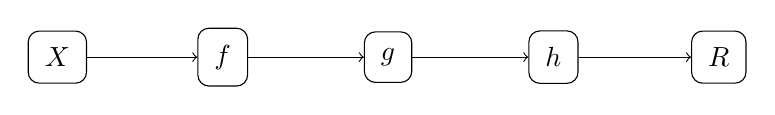
\begin{tikzpicture}[node distance=2.1cm, every node/.style={draw, rounded corners, inner sep=6pt}]
    \node (x) {$X$};
    \node (f) [right of=x] {$f$};
    \node (g) [right of=f] {$g$};
    \node (h) [right of=g] {$h$};
    \node (r) [right of=h] {$R$};
    \draw[->] (x) -- (f);
    \draw[->] (f) -- (g);
    \draw[->] (g) -- (h);
    \draw[->] (h) -- (r);
  \end{tikzpicture}
  \caption{A four-stage workflow with inspectable intermediate boundaries.}
  \label{fig:workflow}
\end{figure}

\section{Evaluation plan}
For each boundary, record the input hash, transformation version, and output
schema. A minimal experiment varies one transformation at a time and compares
the final result with the baseline in Eq.~\eqref{eq:workflow}. The figure is
deliberately generated in TikZ so it can be edited without an external asset.

\section{Conclusion}
The class provides a clean starting point for a mathematics-of-composition
article: author metadata is explicit, the abstract is separated from the body,
and the document includes examples of the common elements an editor needs to
review.

\begin{thebibliography}{1}
\bibitem{wickham2014}
Hadley Wickham. Tidy data. \emph{Journal of Statistical Software}, 59(10),
2014. \href{https://doi.org/10.18637/jss.v059.i10}{doi:10.18637/jss.v059.i10}.
\end{thebibliography}

\end{document}
